\جزوحصہء{رتبہ اور "o" علامتیت}
بڑے \عددی{O} اور چھوٹے \عددی{o} کی علامت کمپیوٹر سائنس میں عام استعمال ہوتی ہے۔ انہیں یہاں متعارف کیا جاتا ہے۔

\ابتدا{تعریف}
اگر \عددی{   x\to\infty} کرتے ہوئے \عددی{\lim_{x\to \infty}\frac{f(x)}{g(x)}=0} ہو تب  ہم کہتے ہیں کہ \عددی{f} کا رتبہ \عددی{g} سے کم ہے جس کو \عددی{f=o(g)}  سے ظاہر کیا جاتا ہے۔ اس کو "\عددی{f}، \عددی{g} کا چھوٹا عددی{o} ہے" پڑھا جاتا ہے۔ 
\انتہا{تعریف}
%===================

یوں \عددی{x\to \infty} کرتے ہوئے \عددی{f=o(g)}  سے مراد \عددی{x\to \infty} کرتے ہوئے \عددی{f} کے بڑھنے کی شرح \عددی{g} سے کم ہے۔

\ابتدا{مثال}
\begin{align*}
\ln x&=o(x) \quad \text{پر}\quad x\to\infty\quad \text{لہٰذا}\quad \lim_{x\to\infty}\frac{\ln x}{x}=0\quad \text{چونکہ}\\
x^2&=o(x^3+1) \quad \text{پر}\quad x\to\infty\quad \text{لہٰذا}\quad \lim_{x\to\infty}\frac{x^2}{x^3+1}=0\quad \text{چونکہ}
\end{align*}
\انتہا{مثال}
%===================
\ابتدا{تعریف}
فرض کریں کافی بڑے \عددی{x} پر \عددی{f(x)} اور \عددی{g(x)} مثبت ہیں۔ تب کافی بڑے  \عددی{x} پر اگر کسی مثبت عدد صحیح \عددی{M} کے لئے
\begin{align*}
\frac{f(x)}{g(x)}\le M
\end{align*}
ہو تب \عددی{x\to\infty} پر \عددی{f} کا رتبہ زیادہ سے زیادہ \عددی{g} کے رتبے جتنا ہو گا۔ اس کو ہم \عددی{f=O(g)} سے ظاہر کرتے ہیں جس
 کو "\عددی{f}، \عددی{g} کا بڑا \عددی{O} ہے' پڑھا جاتا ہے۔
\انتہا{تعریف}
%=====================

\ابتدا{مثال}
چونکہ کافی بڑے \عددی{x} کے لئے \عددی{\frac{x+\sin x}{x}\le 2} ہے لہٰذا \عددی{x\to \infty} پر \عددی{x+\sin x=O(x)} ہو گا۔
\انتہا{مثال}
%=====================
\ابتدا{مثال}
\عددی{x\to\infty} پر \عددی{\frac{e^x+x^2}{e^x}\to 1}  کی بنا \عددی{x\to\infty} پر \عددی{e^x+x^2=O(e^x)} ہو گا۔ اسی طرح 
\عددی{x\to\infty} پر \عددی{\frac{x}{e^x}\to 0}  کی بنا \عددی{x\to\infty} پر \عددی{x=O(e^x)} ہو گا۔
\انتہا{مثال}
%=====================

تعریف پر دوبارہ نظر دوڑاتے ہوئے  آپ دیکھیں گے کہ کافی بڑے \عددی{x} پر مثبت تفاعل کے لئے  \عددی{f=o(g)}سے مراد \عددی{f=O(g)} ہے۔ اس کے علاوہ اگر \عددی{f} اور \عددی{g}  کے بڑھنے کی شرح ایک دوسرے جتنی ہو تب \عددی{f=O(g)} اور \عددی{g=O(f)} ہوں گے (سوال \حوالہ{سوال_ماورائی_ایک_برابر_شرح})۔ 

\جزوحصہ{ترتیبی اور ثنائی تلاش}
کمپیوٹر کسی لائحہ کار کے تحت قدم با قدم چل کر کوئی کام سر انجام دیتا ہے۔اس لائحہ کار کو \اصطلاح{کمپیوٹر الخوارزم}\فرہنگ{الخوارزم!کمپیوٹر}\حاشیہب{computer algorithm}\فرہنگ{algorithm} کہتے ہیں۔اس لائحہ کار کی کارگزاری جاننے کی خاطر ماہرین عموماً اس کام کو سرانجام کرنے کے کئے درکار قدموں کی گنتی کرتے ہیں۔ ایک ہی کام سرانجام دینے کے دو مختلف لائحہ کار کی کارگزاری میں بہت زیادہ فرق ہو سکتا ہے جنہیں بڑے \عددی{O} علامتی روپ میں پیش کیا جاتا ہے۔ آئیں ایک مثال دیکھتے ہیں۔

ایک لغت میں کسی ایک حرف سے شروع ہونے والے الفاظ کی تعداد  \عددی{\num{26000}} ہے۔ آپ اس حرف سے شروع ہونے والے ایک لفظ کو دو طریقوں سے تلاش کر سکتے ہیں۔ پہلی ترکیب میں آپ پہلے لفظ سے شروع کرتے ہوئے ایک ایک لفظ پڑھ کر درکار لفظ تک پہنچتے ہیں۔ اس ترکیب کو \اصطلاح{ترتیبی تلاش}\فرہنگ{تلاش!ترتیبی}\حاشیہب{sequential search}\فرہنگ{search!sequential} کہتے ہیں جو لغت میں ترتیب سے الفاظ لکھے گئے ہونے سے استفادہ نہیں کرتا ہے۔ اس ترتیب میں آپ ہر صورت لفظ تلاش کر پائیں گے (یا جان جائیں گے کہ یہ لفظ لغت میں موجود نہیں ہے) لیکن عین ممکن ہے کہ آپ کو \عددی{\num{26000}} قدم چلنا پڑے۔

اس سے بہتر ترکیب میں آپ لغت کے عین وسط (ایک دو الفاظ آگے پیچھے ہو سکتے ہیں) میں ایک لفظ کو دیکھتے ہیں۔ چونکہ لغت میں الفاظ ترتیب سے ہیں لہٰذا آپ معلوم کر پائیں گے کہ آیا درکار لفظ پہلی نصف یا دوسری نصف حصہ میں ہے۔ لغت کی اس نصف حصہ کو رد کریں جس میں لفظ موجود نہیں ہے۔یوں پہلی قدم میں \عددی{\num{13000}} الفاظ سے چھٹکارا حاصل ہوتا ہے۔  اب منتخب حصہ کے نصف میں جا کر دیکھیں کہ درکار لفظ کس جانب پایا جاتا ہے۔ یوں دوسرے قدم میں \عددی{6500} الفاظ سے چھٹکارا حاصل ہوتا ہے۔ اسی طرح ہر قدم پر آدھے حصے کو رد کرتے ہوئے چلتے جائیں جب تک آپ درکار لفظ تلاش نہیں کر پاتے یا الفاظ ختم نہیں ہو جاتے۔ چونکہ
\begin{align*}
\frac{26000}{2^{15}}<1
\end{align*}
ہوتا ہے لہٰذا  آپ کو زیادہ سے زیادہ \عددی{15} قدم چل کر درکار لفظ مل جائے گا یا آپ جان جائیں گے کہ یہ لفظ لغت میں موجود نہیں ہے۔ اس ترتیب کو \اصطلاح{ثنائی!تلاش}\فرہنگ{ثنائی تلاش}\حاشیہب{binary search}\فرہنگ{search!binary} کہتے ہیں۔

ایک سلسلہ جس کی لمبائی \عددی{n} ہو میں کسی جزو کی تلاش کے لئے ترتیبی تلاش کو \عددی{n} قدم درکار ہو سکتے ہیں۔ اس کے برعکس ثنائی تلاش استعمال کرتے ہوئے  اگر \عددی{2^{m-1}<n<2^m} ہو تب \عددی{m-1<\log_2n\le m} ہو گا اور ایک لفظ تک پہنچنے کی خاطر زیادہ سے زیادہ \عددی{m=\lceil\log_2n\rceil} (\عددی{\log_2n} کا عدد صحیح چھت تفاعل)  بار دو حصوں میں تقسیم کی ضرورت پیش آئے گی۔ یوں ثنائی تلاش میں  \عددی{\log_2 n} کے لگ بھگ  قدم درکار ہوں گے۔ 

بڑے \عددی{O} روپ میں اس تمام کو نہایت خوش اسلوبی سے ظاہر کیا جا سکتا ہے۔ ترتیبی سلسلہ میں ترتیبی تلاش کو \عددی{O(n)} کے لگ بھگ قدم درکار ہوں گے جبکہ ثنائی تلاش کو \عددی{O(\log_2n)} کے لگ بھگ قدم درکار ہوں گے۔ ہماری مثال میں ان دو میں بہت زیادہ فرق پایا جاتا ہے (\عددی{\num{26000}} بالمقابل \عددی{15}) اور چونکہ \عددی{n\to \infty} کرتے ہوئے \عددی{\log_2n} کے لحاظ سے \عددی{n} زیادہ تیزی سے بڑھتا ہے لہٰذا \عددی{n} بڑھانے سے یہ فرق زیادہ بڑھے گا۔


\حصہء{سوالات}
\موٹا{قوت نما \عددی{e^x} کے ساتھ موازنہ}

\ابتدا{سوال}
\عددی{x\to\infty} کرتے ہوئے درج ذیل میں سے کونسا تفاعل \عددی{e^x} سے زیادہ تیزی سے بڑھتا ہے؟ کونسا \عددی{e^x} کی شرح سے بڑھتا ہے؟  کونسا \عددی{e^x} سے کم تیزی سے بڑھتا ہے؟
\begin{multicols}{4}
\begin{enumerate}[a.]
\item
$x+3$
\item
$x^3+\sin^2x$
\item
$\sqrt{x}$
\item
$4^x$
\item
$(\tfrac{3}{2})^x$
\item
$e^{x/2}$
\item
$\frac{e^x}{2}$
\item
$\log_{10}x$
\end{enumerate}
\end{multicols}
جواب:\quad
(ا) آہستہ (ب) آہستہ (ج) آہستہ (د) تیز (ہ) آہستہ  (و) آہستہ (ز) ایک جیسا (ح) آہستہ
\انتہا{سوال}
%======================
\ابتدا{سوال}
\عددی{x\to\infty} کرتے ہوئے درج ذیل میں سے کونسا تفاعل \عددی{e^x} سے زیادہ تیزی سے بڑھتا ہے؟ کونسا \عددی{e^x} کی شرح سے بڑھتا ہے؟  کونسا \عددی{e^x} سے کم تیزی سے بڑھتا ہے؟
\begin{multicols}{4}
\begin{enumerate}[a.]
\item
$10x^4+30x+1$
\item
$x\ln x-x$
\item
$\sqrt{1+x^4}$
\item
$(\tfrac{5}{2})^x$
\item
$e^{-x}$
\item
$xe^x$
\item
$e^{\cos x}$
\item
$e^{x-1}$
\end{enumerate}
\end{multicols}
\انتہا{سوال}
%======================
\موٹا{طاقت \عددی{x^2} کے ساتھ موازنہ}

\ابتدا{سوال}
\عددی{x\to\infty} کرتے ہوئے درج ذیل میں سے کونسا تفاعل \عددی{x^2} سے زیادہ تیزی سے بڑھتا ہے؟ کونسا \عددی{x^2} کی شرح سے بڑھتا ہے؟  کونسا \عددی{x^2} سے کم تیزی سے بڑھتا ہے؟
\begin{multicols}{4}
\begin{enumerate}[a.]
\item
$x^2+4x$
\item
$x^5-x^2$
\item
$\sqrt{x^4+x^3}$
\item
$(x+3)^2$
\item
$x\ln x$
\item
$2^x$
\item
$x^3e^{-x}$
\item
$8x^2$
\end{enumerate}
\end{multicols}
جواب:\quad
(ا) ایک جیسا (ب) تیز (ج) ایک جیسا (د) ایک جیسا (ہ) آہستہ (و) تیز (ز) آہستہ (ح) ایک جیسا 
\انتہا{سوال}
%======================
\ابتدا{سوال}
\عددی{x\to\infty} کرتے ہوئے درج ذیل میں سے کونسا تفاعل \عددی{x^2} سے زیادہ تیزی سے بڑھتا ہے؟ کونسا \عددی{x^2} کی شرح سے بڑھتا ہے؟  کونسا \عددی{x^2} سے کم تیزی سے بڑھتا ہے؟
\begin{multicols}{4}
\begin{enumerate}[a.]
\item
$x^2+\sqrt{x}$
\item
$10x^2$
\item
$x^2e^{-x}$
\item
$\log_{10}(x^2)$
\item
$x^3-x^2$
\item
$(\tfrac{1}{10})^x$
\item
$(1.1)^x$
\item
$x^2+100x$
\end{enumerate}
\end{multicols}
\انتہا{سوال}
%======================
\موٹا{لوگارتھم \عددی{\ln x} کے ساتھ موازنہ}

\ابتدا{سوال}
\عددی{x\to\infty} کرتے ہوئے درج ذیل میں سے کونسا تفاعل \عددی{\ln x} سے زیادہ تیزی سے بڑھتا ہے؟ کونسا \عددی{\ln x} کی شرح سے بڑھتا ہے؟  کونسا \عددی{\ln x} سے کم تیزی سے بڑھتا ہے؟
\begin{multicols}{4}
\begin{enumerate}[a.]
\item
$\log_3x$
\item
$\ln 2x$
\item
$\ln \sqrt{x}$
\item
$\sqrt{x}$
\item
$x$
\item
$5\ln x$
\item
$\frac{1}{x}$
\item
$e^x$
\end{enumerate}
\end{multicols}
جواب:\quad
(ا) ایک جیسا (ب) ایک جیسا (ج) ایک جیسا (د) تیز (ہ) تیز (و) ایک جیسا (ز) آہستہ (ح) تیز 
\انتہا{سوال}
%======================
\ابتدا{سوال}
\عددی{x\to\infty} کرتے ہوئے درج ذیل میں سے کونسا تفاعل \عددی{\ln x} سے زیادہ تیزی سے بڑھتا ہے؟ کونسا \عددی{\ln x} کی شرح سے بڑھتا ہے؟  کونسا \عددی{\ln x} سے کم تیزی سے بڑھتا ہے؟
\begin{multicols}{4}
\begin{enumerate}[a.]
\item
$\log_2(x^2)$
\item
$\log_{10}10x$
\item
$\frac{1}{\sqrt{x}}$
\item
$\frac{1}{x^2}$
\item
$x-2\ln x$
\item
$e^{-x}$
\item
$\ln(\ln x)$
\item
$\ln(2x+5)$
\end{enumerate}
\end{multicols}
\انتہا{سوال}
%======================
\موٹا{شرح نمو کے لحاظ سے منظم کرنا}

\ابتدا{سوال}
\عددی{x\to \infty} کرتے ہوئے شرح نمو کے لحاظ سے منظم کریں۔ کم تر شرح والے تفاعل کو پہلے لکھیں۔ 
\begin{multicols}{4}
\begin{enumerate}[a.]
\item
$e^x$
\item
$x^x$
\item
$(\ln x)^x$
\item
$e^{x/2}$
\end{enumerate}
\end{multicols}
جواب:\quad
د، ا، ج، ب
\انتہا{سوال}
%====================
\ابتدا{سوال}
\عددی{x\to \infty} کرتے ہوئے شرح نمو کے لحاظ سے ترتیب دیں۔ کم تر شرح والے تفاعل کو پہلے لکھیں۔ 
\begin{multicols}{4}
\begin{enumerate}[a.]
\item
$2^x$
\item
$x^2$
\item
$(\ln 2)^x$
\item
$e^x$
\end{enumerate}
\end{multicols}
\انتہا{سوال}
%====================
\موٹا{بڑا \عددی{O} اور چھوٹا \عددی{o}؛ رتبہ}

\ابتدا{سوال}
\عددی{x\to\infty} کرتے ہوئے کونسا درست اور کونسا غلط ہے؟
\begin{multicols}{3}
\begin{enumerate}[a.]
\item
$x=o(x)$
\item
$x=o(x+5)$
\item
$x=O(x+5)$
\item
$x=O(2x)$
\item
$e^x=o(e^{2x})$
\item
$x+\ln x=O(x)$
\item
$\ln x=o(\ln 2x)$
\item
$\sqrt{x^2+5}=O(x)$
\end{enumerate}
\end{multicols}
جواب:\quad
(ا) غلط (ب) غلط (ج) درست (د) درست (ہ) درست (و) درست (ز) غلط (ح) درست
\انتہا{سوال}
%============
\ابتدا{سوال}
\عددی{x\to\infty} کرتے ہوئے کونسا درست اور کونسا غلط ہے؟
\begin{multicols}{3}
\begin{enumerate}[a.]
\item
$\frac{1}{x+3}=O(\tfrac{1}{x})$
\item
$\frac{1}{x}+\frac{1}{x^2}=O(\tfrac{1}{x})$
\item
$\frac{1}{x}-\frac{1}{x^2}=o(\tfrac{1}{x})$
\item
$2+\cos x=O(2)$
\item
$e^x+x=O(e^x)$
\item
$x\ln x=o(x^2)$
\item
$\ln(\ln x)=O(\ln x)$
\item
$\ln x=o(\ln(x^2+1))$
\end{enumerate}
\end{multicols}
\انتہا{سوال}
%============
\ابتدا{سوال}\شناخت{سوال_ماورائی_ایک_برابر_شرح}
دکھائیں کہ اگر \عددی{x\to\infty} کرنے سے \عددی{f(x)} اور \عددی{g(x)} کے بڑھنے کی شرح برابر ہو تب \عددی{f=O(g)} اور \عددی{g=O(f)} ہوں گے۔
\انتہا{سوال}
%======================
\ابتدا{سوال}
\عددی{x\to \infty} کرتے ہوئے کب کثیر رکنی \عددی{f(x)} کا رتبہ کثیر رکنی \عددی{g(x)} کے رتبہ سے کم ہو گا؟ اپنے جواب کی وجہ پیش کریں۔
\انتہا{سوال}
%===================
\ابتدا{سوال}
\عددی{x\to \infty} کرتے ہوئے کب کثیر رکنی \عددی{f(x)} کا رتبہ زیادہ سے زیادہ کثیر رکنی \عددی{g(x)} کے رتبہ کے برابر ہو گا؟ اپنے جواب کی وجہ پیش
 کریں۔\\
جواب:\quad
جب \عددی{f} کا درجہ \عددی{g} کے درجہ سے کم یا اس کے برابر ہو۔
\انتہا{سوال}
%=====================
\ابتدا{سوال}\ترچھا{قاعدہ سمسن اور قاعدہ ذوزنقہ}\\
موجودہ حصہ میں پیش کی گئی تعریف کو زیادہ عمومی بنانے کی خاطر ہم اس میں \عددی{x\to\infty} کی پابندی ختم کر کے اس  کی بجائے \عددی{x\to a} پر حد لیتے ہیں جہاں \عددی{a} حقیقی عدد ہے۔ دکھائیں کہ قاعدہ سمسن سے حاصل قطعی تکمل کی تخمین میں \عددی{h\to 0} کرتے ہوئے خلل \عددی{O(h^4)} ہو گا جبکہ قاعدہ ذوزنقہ سے حاصل تخمین میں خلل \عددی{O(h^2)} ہو گا۔ یوں ان دو تراکیب کے نتائج کی درستگی کو اس طرح بھی بیان کیا جا سکتا ہے۔  
\انتہا{سوال}
%===================
\موٹا{دیگر موازنے}

\ابتدا{سوال}
ناطق تفاعل کے حد کے بارے میں حصہ \حوالہ{حصہ_استعمال_تفرق_حد_متقارب_اور_غالب_اجزاء} میں حاصل نتیجہ ہمیں \عددی{x\to \infty} کی صورت میں کثیر رکنی کی اضافی  شرح نمو کے بارے میں کیا بتاتا ہے؟\\
جواب:\quad
زیادہ درجے کا کثیر رکنی، کم درجے کے کثیر رکنی سے زیادہ تیز بڑھتا ہے۔ ایک جیسے درجہ کے کثیر رکنی کی شرح نمو برابر ہوتی ہے۔
\انتہا{سوال}
%=======================
\ابتدا{سوال}\ترچھا{کمپیوٹر ترسیم}\\
(ا) درج ذیل پر تحقیق کریں۔ اس کے بعد قاعدہ لھوپیٹال سے اس تحقیق سے حاصل معلومات کی وجہ بیان کریں۔
\begin{align*}
\lim_{x\to\infty}\frac{\ln(x+1)}{\ln x},\quad \lim_{x\to \infty}\frac{\ln(x+999)}{\ln x}
\end{align*}
(ب) دکھائیں کہ درج ذیل کی قیمت ، مستقل\عددی{a} کی قیمت پر منحصر نہیں ہے۔ اس سے تفاعل \عددی{f(x)=\ln(x+a)} اور \عددی{g(x)=\ln x} کے اضافی شرح نمو کے بارے میں کیا کہا جا سکتا ہے؟
\begin{align*}
\lim_{x\to\infty}\frac{\ln(x+a)}{\ln x}
\end{align*}
\انتہا{سوال}
%=============================
\ابتدا{سوال}
دکھائیں کہ \عددی{x\to \infty} کرتے ہوئے \عددی{\sqrt{10x+1}} اور \عددی{\sqrt{x+1}} کی شرح نمو ایک دوسرے کے برابر ہیں۔ یہ دکھانے کی خاطر دکھائیں کہ دونوں تفاعل کی شرح نمو تفاعل \عددی{\sqrt{x}} کے شرح نمو کے برابر ہے۔ 
\انتہا{سوال}
%====================
\ابتدا{سوال}
دکھائیں کہ \عددی{x\to \infty} کرتے ہوئے \عددی{\sqrt{x^4+x}} اور \عددی{\sqrt{x^4-x^3}} کی شرح نمو ایک دوسرے کے برابر ہیں۔ یہ دکھانے کی خاطر دکھائیں کہ دونوں تفاعل کی شرح نمو تفاعل \عددی{x^2} کے شرح نمو کے برابر ہے۔ 
\انتہا{سوال}
%====================
\ابتدا{سوال}\شناخت{سوال_ماورائی_قوت_نمائی_کثیر_رکنی_سے_تیز}
دکھائیں کہ \عددی{x\to \infty} کرتے ہوئے \عددی{e^x} کی شرح نمو کسی بھی \عددی{x^n} کے شرح نمو سے زیادہ ہو گی، جہاں \عددی{n} کوئی بھی مثبت عدد صحیح ہو سکتا ہے، مثلاً \عددی{x^{\num{1000000}}}۔ (اشارہ۔ \عددی{x^n} کا \عددی{n} واں تفرق کیا ہے؟)
\انتہا{سوال}
%=================
\ابتدا{سوال}\ترچھا{تفاعل \عددی{e^x} ہر کثیر رکنی سے زیادہ تیزی سے بڑھتا ہے}\\
دکھائیں کہ \عددی{x\to\infty} کرتے ہوئے \عددی{e^x} کسی بھی کثیر رکنی \عددی{a_nx^n+a_{n-1}x^{n-1}+\cdots+a_1x+a_0} سے زیادہ تیزی سے بڑھتا ہے۔
\انتہا{سوال}
%====================
\ابتدا{سوال}\شناخت{سوال_ماورائی_لوگارتھم_سب_سے_آہستہ}
\begin{enumerate}[a.]
\item
دکھائیں کہ کسی بھی مثبت عدد صحیح \عددی{n} کی صورت میں \عددی{x\to \infty} کرتے ہوئے \عددی{\ln x} کی شرح نمو تفاعل \عددی{x^{1/n}} (مثلاً \عددی{x^{1/\num{1000000}}}) کی شرح نمو سے کم ہو گی۔
\item
اگرچہ \عددی{x^{1/\num{1000000}}} کی قیمت آخر کار \عددی{\ln x} کی قیمت سے زیادہ ہو گی، وہاں تک پہنچنے کے لئے آپ کو محور \عددی{x} پر بہت دور جانا ہو گا۔ ایسا \عددی{x>1} تلاش کریں جس پر \عددی{x^{1/{\num{1000000}}}>\ln x} ہو۔ دھیان رہے کہ \عددی{x>1} کی صورت میں مساوات \عددی{\ln x=x^{1/\num{1000000}}} کو \عددی{\ln(\ln x)=\tfrac{\ln x}{\num{1000000}}} بھی لکھا جا سکتا ہے۔
\item
تفاعل \عددی{x^{1/10}} کو بھی \عددی{\ln x} سے بڑھنے  کے لئے  بہت وقت درکار ہو گا۔ کیلکولیٹر استعمال کرتے ہوئے \عددی{x} کی وہ قیمت تلاش کریں جس پر \عددی{x^{1/10}} کی ترسیم \عددی{\ln x} کی ترسیم کو کٹ کرتی ہو یا جہاں \عددی{\ln x=10\ln(\ln x)} ہو۔
\item
وہ نقطہ جس پر \عددی{\ln x=10\ln(\ln x)} ہو کے قریب اس مساوات  کو کمپیوٹر پر ترسیم کر کے \عددی{x} تلاش کریں۔
\end{enumerate}
جواب:\quad
(ب) 
$\ln(e^{\num{17000000}})=\num{17000000}<(e^{17\times 10^6})^{1/10^6}=e^{17}\approx \num{24154952.75}$\\
(ج)  \عددی{x\approx 3.4306311\times 10^{15}}، (د) نقطہ تقاطع \عددی{x\approx 3.4306311\times 10^{15}} ہے۔
\انتہا{سوال}
%===================
\ابتدا{سوال}\ترچھا{تفاعل \عددی{\ln x} کی شرح نمو ہر کثیر رکنی سے کم ہے}\\
دکھائیں کہ \عددی{x\to\infty} کرتے ہوئے \عددی{\ln x} کی شرح نمو کسی بھی غیر مستقل کثیر رکنی سے کم ہو گی۔
\انتہا{سوال}
%===================
\موٹا{الخوارزم اور تلاش}\\

\ابتدا{سوال}\شناخت{سوال_ماورائی_تلاش_کی_قدمیں}
(ا) آپ کمپیوٹر کی مدد سے ایک کام سرانجام دینا چاہتے ہیں۔ آپ کے پاس تین الخوارزم موجود ہیں جن  کے لئے کمپیوٹر کو درکار   قدموں کی تعداد  درج ذیل تفاعل دیتے ہیں۔ \عددی{n} کی بڑی قیمت کی صورت میں ان میں سے کونسا الخوارزم  بہترین ہے؟ اپنے جواب کی وجہ پیش کریں۔
\begin{align*}
n\log_2n,\quad n^{3/2},\quad n(\log_2n)^2
\end{align*}
(ب) جزو-الف میں دیے گئے تفاعل کو ایک ساتھ ترسیم کرتے ہوئے دیکھیں کونسا زیادہ تیزی سے بڑھتا ہے۔\\
جواب:\quad
(ا) جو \عددی{O(n\log_2n)} قدم چلتا ہے۔
\انتہا{سوال}
%====================
\ابتدا{سوال}
درج ذیل تفاعل کے لئے سوال \حوالہ{سوال_ماورائی_تلاش_کی_قدمیں} کو دہرائیں۔
\begin{align*}
n,\quad \sqrt{n}\log_2n,\quad (\log_2n)^n
\end{align*}
\انتہا{سوال}
%=====================
\ابتدا{سوال}
ایک مرتب سلسلہ جس میں دس لاکھ اجزاء پائے جاتے ہیں میں سے آپ کو ایک جزو تلاش کرنا ہے۔ ترتیبی تلاش کے لئے کتنے قدم درکار ہوں گے؟ ثنائی تلاش کے لئے کتنے قدم درکار ہوں گے؟\\
جواب:\quad
ترتیبی تلاش کو دس لاکھ قدم چلنا پڑھ سکتا ہے جبکہ ثنائی تلاش میں زیادہ سے زیادہ \عددی{20} قدم چلنا ہو گا۔
\انتہا{سوال}
%=================
\ابتدا{سوال}
ایک مرتب سلسلہ میں \عددی{\num{450000}} اجزاء پائے جاتے ہیں جن میں سے آپ کو ایک جزو کی تلاش ہے۔ ترتیبی تلاش اور ثنائی تلاش کرتے ہوئے کتنے قدم درکار ہوں گے؟
\انتہا{سوال}
%===================

\حصہ{الٹ تکونیاتی تفاعل}
الٹ تکونی تفاعل کی ضرورت اس وقت پیش آتی ہے جب ہم مثلث کے ضلع کو ناپ کر زاویہ تلاش کرنا چاہتے ہیں۔ یہ تفاعل اہم الٹ تفرق بھی مہیا کرتے ہیں اور تفرقی مساوات کے حل میں عموماً پائے جاتے ہیں۔ اس حصہ میں ان تفاعل کی تعریف پیش کی جائے گی، ان کو ترسیم کرنا سکھایا جائے گا اور ان کی قیمت حاصل کرنا سکھایا جائے گا۔

\جزوحصہء{الٹ تکونیاتی  کی تعریف}
چھ بنیادی تکونیاتی تفاعل کی قیمتیں دہراتی ہیں لہٰذا یہ ایک ایک تفاعل نہیں ہیں البتہ ان کے دائرہ کار کو ایسے وقفوں پر پابند کیا جا سکتا ہے جہاں یہ ایک ایک ہوں (جدول \حوالہ{جدول_ماورائی_تکونیاتی_تفاعل_ایک_ایک})۔
\begin{table}
\caption{تکونیاتی تفاعل کو ایک ایک بنانے کی خاطر دائرہ کار کو محدود کیا گیا ہے۔}
\label{جدول_ماورائی_تکونیاتی_تفاعل_ایک_ایک}
\centering
\renewcommand{\arraystretch}{2} 
\begin{tabular}{LLL}
\toprule
\text{تفاعل}&\text{\RL{دائرہ کار}}&\text{سعت}\\
\midrule
\sin x&[-\tfrac{\pi}{2},\tfrac{\pi}{2}]&[-1,1]\\
\cos x&[0,\pi]&[-1,1]\\
\tan x&(-\tfrac{\pi}{2},\tfrac{\pi}{2})&(-\infty,\infty)\\
\cot x&(0,\pi)&(-\infty,\infty)\\
\sec x&[0,\tfrac{\pi}{2})\cup (\tfrac{\pi}{2},\pi]&(-\infty,-1]\cup[1,\infty)\\
\csc x&[-\tfrac{\pi}{2},0)\cup(0,\tfrac{\pi}{2}]&(-\infty,-1]\cup[1,\infty)\\
\bottomrule
\end{tabular}
\end{table}

چونکہ محدود دائرہ کار والے تکونیاتی تفاعل ایک ایک ہیں لہٰذا ان کا الٹ پائے جاتے ہیں جنہیں ظاہر کرنا کا طریقہ درج ذیل ہے۔
\begin{align*}
y&=\sin^{-1}x\\
y&=\cos^{-1}x\\
y&=\tan^{-1}x\\
y&=\cot^{-1}x\\
y&=\sec^{-1}x\\
y&=\csc^{-1}x
\end{align*}
ہم کہیں گے "\عددی{x} کا الٹ سائن \عددی{y} کے برابر ہے"، وغیرہ۔ یاد رہے کہ ان الٹ تفاعل میں \عددی{-1} سے مراد الٹ تفاعل ہے اور لہٰذا اس کو ہرگز بالعکس متناسب تصور نہیں کیا جائے۔ مثال کے طور پر \عددی{\sin x} کا بالعکس متناسب \عددی{(\sin x)^{-1}=\tfrac{1}{\sin x}=\csc x} ہو گا۔

الٹ تکونیاتی تفاعل کے دائرہ کار یوں منتخب کئے جاتے ہیں کہ درج ذیل مطمئن ہوں۔
\begin{align}
\sec^{-1}x&=\cos^{-1}(1/x)\\
\csc^{-1}x&=\sin^{-1}(1/x)\\
\cot^{-1}x&=\tfrac{\pi}{2}-\tan^{-1}x
\end{align}

ان تعلقات کو استعمال کر کے \عددی{\cos^{-1}x}، \عددی{\sin^{-1}x} اور \عددی{\tan^{-1}x} کی قیمتیں جانتے ہوئے ہم بالترتیب \عددی{\sec^{-1}x}، \عددی{\csc^{-1}x} اور \عددی{\cot^{-1}x} کی قیمتیں معلوم کر سکتے ہیں۔

\جزوحصہء{الٹ سائن اور الٹ کوسائن}
 متغیر \عددی{x} کے الٹ سائن یعنی \عددی{\sin^{-1}x} سے مراد وہ زاویہ ہے جس کا سائن \عددی{x} کے برابر ہو۔ اسی طرح \عددی{\cos^{-1}x} سے مراد وہ زاویہ ہے جس کے کوسائن کی قیمت \عددی{x} ہو۔

\ابتدا{تعریف}
\عددی{y=\sin^{-1}x} سے مراد وقفہ \عددی{[-\pi/2,\pi/2]} میں وہ عدد \عددی{y} ہے جس کے لئے \عددی{\sin y=x} ہو۔ اسی طرح 
\عددی{y=\cos^{-1}x} سے مراد وقفہ \عددی{[0,\pi]} میں وہ عدد \عددی{y} ہے جس کے لئے \عددی{\cos y=x} ہو۔
\انتہا{تعریف}
%=============

تفاعل \عددی{y=\sin^{-1}x} (شکل \حوالہ{شکل_ماورائی_سائن_اور_الٹ_سائن}) کی ترسیم مبدا کے لحاظ سے تشاکلی ہے (اور عین \عددی{x=\sin y} کی ترسیم پر پائی جاتی ہے)۔ یوں الٹ سائن طاق تفاعل ہے:
\begin{align}\label{مساوات_ماورائی_الٹ_سائن_تعلق}
\sin^{-1}(-x)=-\sin^{-1}x
\end{align}
تفاعل \عددی{y=\cos^{-1}x} (شکل \حوالہ{شکل_ماورائی_کوسائن_اور_الٹ_کوسائن}) کی ترسیم میں ایسی کوئی تشاکلی نہیں پائی جاتی ہے۔
\begin{figure}
\centering
\begin{subfigure}{0.45\textwidth}
\centering
\begin{tikzpicture}[font=\small,declare function={f(\x)=sin(deg(\x));}]
\pgfmathsetmacro{\k}{pi/2}
\begin{axis}[clip=false,small,axis lines=middle,xlabel={$x$},ylabel={$y$},xlabel style={at={(current axis.right of origin)},anchor=west},ylabel style={at={(current axis.above origin)},anchor=south},xtick={-\k,\k},xticklabels={$-\tfrac{\pi}{2}$,$\tfrac{\pi}{2}$},ytick={-1,1},enlargelimits=true]
\addplot[domain=-\k:\k,smooth]{f(x)};
\addplot[dashed,domain=-\k:-\k-1,smooth]{f(x)};
\addplot[dashed,domain=\k:\k+1,smooth]{f(x)};
\draw(-0.5,0.5)node[left,font=\scriptsize]{$\begin{aligned}y=\sin x,\, -\tfrac{\pi}{2}\le x\le \tfrac{\pi}{2}\\ [-\pi/2,\pi/2]\quad \text{\RL{دائرہ کار:}} \\ 
[-1,1] \quad \text{سعت:}   \end{aligned}$};
\draw(\k,{f(\k)})node[circ]{};
\draw(-\k,{f(-\k)})node[circ]{};
\end{axis}
\end{tikzpicture}
\caption{}
\end{subfigure}\hfill
\begin{subfigure}{0.45\textwidth}
\centering
\begin{tikzpicture}[font=\small,declare function={f(\x)=sin(deg(\x));}]
\pgfmathsetmacro{\k}{pi/2}
\begin{axis}[clip=false,small,axis lines=middle,xlabel={$x$},ylabel={$y$},xlabel style={at={(current axis.right of origin)},anchor=west},ylabel style={at={(current axis.above origin)},anchor=south},ytick={-\k,\k},yticklabels={$-\tfrac{\pi}{2}$,$\tfrac{\pi}{2}$},xtick={-1,1},enlargelimits=true]
\addplot[domain=-\k:\k,smooth]({f(x)},x);
\addplot[dashed,domain=-\k:-\k-1,smooth]({f(x)},x);
\addplot[dashed,domain=\k:\k+1,smooth]({f(x)},x)node[above]{$x=\sin y$};
\draw(-0.25,1.5)node[left,font=\scriptsize]{$\begin{aligned}y=\sin^{-1} x\\ [-1,1]\quad \text{\RL{دائرہ کار:}} \\ [-\pi/2,\pi/2]\quad \text{\RL{سعت:}} \end{aligned}$};
\draw({f(\k)},\k)node[circ]{};
\draw({f(-\k)},-\k)node[circ]{};
\end{axis}
\end{tikzpicture}
\caption{}
\end{subfigure}
\caption{
ترسیمات برائے (ا) \عددی{y=\sin x,\,-\pi/2\le x\le \pi/2}  اور (ب)  الٹ سائن تفاعل \عددی{y=\sin^{-1}x}؛ لکیر \عددی{y=x} میں عکس \عددی{\sin^{-1}x} درحقیقت قوس \عددی{x=\sin y} کا کچھ حصہ ہے۔
}
\label{شکل_ماورائی_سائن_اور_الٹ_سائن}
\end{figure}
%
\begin{figure}
\centering
\begin{subfigure}{0.45\textwidth}
\centering
\begin{tikzpicture}[font=\small,declare function={f(\x)=cos(deg(\x));}]
\pgfmathsetmacro{\k}{pi}
\pgfmathsetmacro{\kh}{pi/2}
\begin{axis}[clip=false,small,axis lines=middle,xlabel={$x$},ylabel={$y$},xlabel style={at={(current axis.right of origin)},anchor=west},ylabel style={at={(current axis.above origin)},anchor=south},xtick={\kh,\k},xticklabels={$-\tfrac{\pi}{2}$,$\pi$},ytick={-1,1},enlargelimits=true]
\addplot[domain=0:\k,smooth]{f(x)};
\addplot[dashed,domain=0:-1,smooth]{f(x)};
\addplot[dashed,domain=\k:\k+1,smooth]{f(x)};
\draw(0.75,0.5)node[right,font=\scriptsize]{$\begin{aligned}y=\cos x,\, 0\le x\le \pi\\ [0,\pi]\quad \text{\RL{دائرہ کار:}} \\ 
[-1,1] \quad \text{سعت:}   \end{aligned}$};
\draw(0,{f(0)})node[circ]{};
\draw(\k,{f(\k)})node[circ]{};
\end{axis}
\end{tikzpicture}
\caption{}
\end{subfigure}\hfill
\begin{subfigure}{0.45\textwidth}
\centering
\begin{tikzpicture}[font=\small,declare function={f(\x)=cos(deg(\x));}]
\pgfmathsetmacro{\k}{pi}
\pgfmathsetmacro{\kh}{pi/2}
\begin{axis}[clip=false,small,axis lines=middle,xlabel={$x$},ylabel={$y$},xlabel style={at={(current axis.right of origin)},anchor=west},ylabel style={at={(current axis.above origin)},anchor=south},ytick={\kh,\k},yticklabels={$\tfrac{\pi}{2}$,$\pi$},xtick={-1,1},enlargelimits=true]
\addplot[domain=0:\k,smooth]({f(x)},x);
\addplot[dashed,domain=0:-1,smooth]({f(x)},x);
\addplot[dashed,domain=\k:\k+1,smooth]({f(x)},x)node[above]{$x=\cos y$};
\draw(0.25,\k)node[right,font=\scriptsize]{$\begin{aligned}y=\cos^{-1} x\\ [-1,1]\quad \text{\RL{دائرہ کار:}} \\ 
[0,\pi]\quad \text{\RL{سعت:}} \end{aligned}$};
\draw({f(0)},0)node[circ]{};
\draw({f(\k)},\k)node[circ]{};
\end{axis}
\end{tikzpicture}
\caption{}
\end{subfigure}
\caption{
ترسیمات برائے (ا) \عددی{y=\cos x,\,0\le x\le \pi}  اور (ب) الٹ کوسائن تفاعل \عددی{y=\cos^{-1}x}؛ لکیر \عددی{y=x} میں عکس \عددی{\cos^{-1}x} درحقیقت قوس \عددی{x=\cos y} کا کچھ حصہ ہے۔
}
\label{شکل_ماورائی_کوسائن_اور_الٹ_کوسائن}
\end{figure}


\ابتدا{مثال}\شناخت{مثال_ماورائی_سائن_مخصوص_قیمتیں}\ترچھا{تفاعل \عددی{\sin^{-1}x} کی مخصوص قیمتیں}\\
\begin{figure}
\centering
\begin{subfigure}{0.45\textwidth}
\centering
\begin{tikzpicture}[font=\scriptsize]
\pgfmathsetmacro{\r}{1.25}
\pgfmathsetmacro{\ang}{60}
\draw[-latex](-1.5,0)--(1.5,0)node[right]{$x$};
\draw[-latex](0,-1.4)--(0,1.5)node[above]{$y$};
\draw[opacity=0.5,fill=lgray]([shift={(90:\r)}]0,0) arc (90:270:\r);
\draw([shift={(-90:\r)}]0,0) arc (-90:90:\r);
\draw(0,0)--++(\ang:\r)node[pos=0.5,above left,xshift=1ex]{$2$}coordinate[](kT)--($(0,0)!(kT)!(1.25,0)$)coordinate[](kR)node[pos=0.6,right,xshift=-0.5ex]{$\sqrt{3}$};
\draw($(0,0)!0.5!(kR)$)node[below]{$1$};
\draw[-stealth]([shift={(0:0.3)}]0,0) arc (0:\ang:0.3);
\draw(\ang/2:0.5)node[]{$\tfrac{\pi}{3}$};
\draw(45:\r)node[above right]{$\sin^{-1}\frac{\sqrt{3}}{2}=\frac{\pi}{3}$};
\draw(-45:\r)node[below right]{$\sin\frac{\pi}{3}=\frac{\sqrt{3}}{2}$};
\end{tikzpicture}
\end{subfigure}\hfill
\begin{subfigure}{0.45\textwidth}
\centering
\begin{tikzpicture}[font=\scriptsize]
\pgfmathsetmacro{\r}{1.25}
\pgfmathsetmacro{\ang}{-45}
\draw[-latex](-1.5,0)--(1.5,0)node[right]{$x$};
\draw[-latex](0,-1.4)--(0,1.5)node[above]{$y$};
\draw[opacity=0.5,fill=lgray]([shift={(90:\r)}]0,0) arc (90:270:\r);
\draw([shift={(-90:\r)}]0,0) arc (-90:90:\r);
\draw(0,0)--++(\ang:\r)node[pos=0.5,below left,xshift=1ex]{$\sqrt{2}$}coordinate[](kT)--($(0,0)!(kT)!(1.25,0)$)coordinate[](kR)node[pos=0.7,right,xshift=-0.5ex,font=\tiny]{$-1$};
\draw($(0,0)!0.5!(kR)$)node[above]{$1$};
\draw[-stealth]([shift={(0:0.3)}]0,0) arc (0:\ang:0.3);
\draw(\ang/2:0.6)node[]{$-\tfrac{\pi}{4}$};
\draw(60:\r)node[above right]{$\sin^{-1}(\frac{1}{\sqrt{2}})=\sin^{-1}(-\frac{\sqrt{2}}{2})=-\frac{\pi}{4}$};
\draw(-60:\r)node[below right]{$\sin(-\frac{\pi}{4})=-\frac{1}{\sqrt{2}}$};
\end{tikzpicture}
\end{subfigure}
\caption{سائن اور الٹ سائن کی مخصوص قیمتیں (مثال \حوالہ{مثال_ماورائی_سائن_مخصوص_قیمتیں})۔}
\label{شکل_مثال_ماورائی_سائن_مخصوص_قیمتیں}
\end{figure}

الٹ سائن کی مخصوص قیمتوں کو قائمہ مثلث سے شکل \حوالہ{مثال_ماورائی_سائن_مخصوص_قیمتیں} میں حاصل کرنا دکھایا گیا ہے۔ اس طرح درج ذیل دیگر قیمتیں بھی حاصل کی جا سکتی ہیں۔ یاد رہے کہ \عددی{\sin^{-1}x} کا سعت \عددی{[-\tfrac{\pi}{2},\tfrac{\pi}{2}]} ہے  لہٰذا زاویے ربع اول اور ربع چہارم میں پائے جائیں گے۔
\begin{align*}
\renewcommand{\arraystretch}{2} 
\begin{array}{c|cccccc}
x&\tfrac{\sqrt{3}}{2}&\tfrac{\sqrt{2}}{2}&\tfrac{1}{2}&-\tfrac{1}{2}&-\tfrac{\sqrt{2}}{2}&-\tfrac{\sqrt{3}}{2}\\
\hline
\sin^{-1}x&\tfrac{\pi}{3}&\tfrac{\pi}{4}&\tfrac{\pi}{6}&-\tfrac{\pi}{6}&-\tfrac{\pi}{4}&-\tfrac{\pi}{3}
\end{array}
\end{align*}
\انتہا{مثال}
%=====================

\ابتدا{مثال}\شناخت{مثال_ماورائی_کوسائن_مخصوص_قیمتیں}\ترچھا{تفاعل \عددی{\cos^{-1}x} کی مخصوص قیمتیں}\\
\begin{figure}
\centering
\begin{subfigure}{0.45\textwidth}
\centering
\begin{tikzpicture}[font=\scriptsize]
\pgfmathsetmacro{\r}{1.25}
\pgfmathsetmacro{\ang}{45}
\draw[-latex](-1.5,0)--(1.5,0)node[right]{$x$};
\draw[-latex](0,-1.4)--(0,1.5)node[above]{$y$};
\draw[opacity=0.5,fill=lgray]([shift={(180:\r)}]0,0) arc (180:360:\r);
\draw([shift={(0:\r)}]0,0) arc (0:180:\r);
\draw(0,0)--++(\ang:\r)node[pos=0.5,above left,xshift=1ex]{$\sqrt{2}$}coordinate[](kT)--($(0,0)!(kT)!(1.25,0)$)coordinate[](kR)node[pos=0.6,right,xshift=-0.5ex]{$1$};
\draw($(0,0)!0.5!(kR)$)node[below]{$1$};
\draw[-stealth]([shift={(0:0.3)}]0,0) arc (0:\ang:0.3);
\draw(\ang/2:0.5)node[]{$\tfrac{\pi}{4}$};
\draw(45:\r)node[above right]{$\cos^{-1}\frac{1}{\sqrt{2}}=\cos^{-1}\frac{\sqrt{2}}{2}=\frac{\pi}{4}$};
\draw(-45:\r)node[below right]{$\cos\frac{\pi}{4}=\frac{1}{\sqrt{2}}$};
\end{tikzpicture}
\end{subfigure}\hfill
\begin{subfigure}{0.45\textwidth}
\centering
\begin{tikzpicture}[font=\scriptsize]
\pgfmathsetmacro{\r}{1.25}
\pgfmathsetmacro{\ang}{120}
\draw[-latex](-1.5,0)--(1.5,0)node[right]{$x$};
\draw[-latex](0,-1.4)--(0,1.5)node[above]{$y$};
\draw[opacity=0.5,fill=lgray]([shift={(180:\r)}]0,0) arc (180:360:\r);
\draw([shift={(0:\r)}]0,0) arc (0:180:\r);
\draw(0,0)--++(\ang:\r)node[pos=0.5,above right,xshift=-1ex]{$2$}coordinate[](kT)--($(0,0)!(kT)!(1.25,0)$)coordinate[](kR)node[pos=0.7,left,xshift=0.5ex]{$\sqrt{3}$};
\draw($(0,0)!0.5!(kR)$)node[below,xshift=-0.5ex]{$-1$};
\draw[-stealth]([shift={(0:0.3)}]0,0) arc (0:\ang:0.3);
\draw(\ang/3:0.6)node[]{$\tfrac{2\pi}{3}$};
\draw(60:\r)node[above right]{$\cos^{-1}(-\frac{1}{2})=\frac{2\pi}{3}$};
\draw(-60:\r)node[below right]{$\cos(\frac{2\pi}{3})=-\frac{1}{2}$};
\end{tikzpicture}
\end{subfigure}
\caption{کوسائن اور الٹ سائن کی مخصوص قیمتیں (مثال \حوالہ{مثال_ماورائی_کوسائن_مخصوص_قیمتیں})۔}
\label{شکل_مثال_ماورائی_کوسائن_مخصوص_قیمتیں}
\end{figure}

الٹ کوسائن کی مخصوص قیمتوں کو قائمہ مثلث سے شکل \حوالہ{مثال_ماورائی_کوسائن_مخصوص_قیمتیں} میں حاصل کرنا دکھایا گیا ہے۔ اس طرح درج ذیل دیگر قیمتیں بھی حاصل کی جا سکتی ہیں۔ یاد رہے کہ \عددی{\cos^{-1}x} کا سعت \عددی{[0,\pi]} ہے  لہٰذا زاویے ربع اول اور ربع دوم میں پائے جائیں گے۔
\begin{align*}
\renewcommand{\arraystretch}{2} 
\begin{array}{c|cccccc}
x&\tfrac{\sqrt{3}}{2}&\tfrac{\sqrt{2}}{2}&\tfrac{1}{2}&-\tfrac{1}{2}&-\tfrac{\sqrt{2}}{2}&-\tfrac{\sqrt{3}}{2}\\
\hline
\cos^{-1}x&\tfrac{\pi}{6}&\tfrac{\pi}{4}&\tfrac{\pi}{3}&\tfrac{2\pi}{3}&\tfrac{3\pi}{4}&\tfrac{5\pi}{6}
\end{array}
\end{align*}
\انتہا{مثال}
%=====================
\جزوحصہء{تماثل جن میں الٹ سائن اور الٹ کوسائن پائے جاتے ہوں}
ہم شکل \حوالہ{شکل_ماورائی_کوسائن_اور_الٹ_کوسائن_تعلق} میں دیکھتے ہیں کہ \عددی{x} کا الٹ کوسائن تماثل
\begin{align}\label{مساوات_ماورائی_تماثل_الف}
\cos^{-1}x+\cos^{-1}(-x)=\pi
\end{align}
کو مطمئن کرتا ہے جس کو درج ذیل بھی لکھا جا سکتا ہے۔
\begin{align}\label{مساوات_ماورائی_تماثل_ب}
\cos^{-1}(x)=\pi-\cos^{-1}x
\end{align}
اسی طرح شکل \حوالہ{شکل_ماورائی_سائن_کوسائن_تعلق} میں مثلث کو دیکھ کر درج ذیل لکھا جا سکتا ہے۔
\begin{align}\label{مساوات_ماورائی_تماثل_ج}
\sin^{-1}x+\cos^{-1}x=\frac{\pi}{2}
\end{align}
اگرچہ شکل \حوالہ{شکل_ماورائی_سائن_کوسائن_تعلق} میں دی گئی مثلث سے یہ ثابت نہیں کیا جا سکتا ہے لیکن مساوات \حوالہ{مساوات_ماورائی_تماثل_ج} وقفہ \عددی{[-1,1]} میں دیگر \عددی{x} کے لئے بھی درست ہے۔ یہ حقیقت البتہ مساوات \حوالہ{مساوات_ماورائی_الٹ_سائن_تعلق} اور مساوات \حوالہ{مساوات_ماورائی_تماثل_ب} کا نتیجہ ہے۔
\begin{figure}
\centering
\begin{minipage}{0.45\textwidth}
\centering
\begin{tikzpicture}[font=\scriptsize]
\pgfmathsetmacro{\r}{1.25}
\pgfmathsetmacro{\ang}{45}
\pgfmathsetmacro{\angC}{180-\ang}
\draw[-latex](-1.5,0)--(1.75,0)node[right]{$x$};
\draw[-latex](0,-1.4)--(0,1.5)node[above]{$y$};
\draw[opacity=0.5,fill=lgray]([shift={(180:\r)}]0,0) arc (180:360:\r);
\draw([shift={(0:\r)}]0,0) arc (0:180:\r);
\draw(0,0)--++(\ang:\r)coordinate[](kT)--($(0,0)!(kT)!(1.25,0)$)coordinate[](kR)node[below]{$x$};
\draw[-stealth]([shift={(0:0.3)}]0,0) arc (0:\ang:0.3);
\draw(-\r,0)node[below,xshift=-1.5ex]{$-1$} (\r,0)node[below,xshift=1ex]{$1$};
\draw(\ang/2:0.4)--++(\ang/2:1)node[right]{$\cos^{-1}x$};
\draw(0,0)--++(\angC:\r)coordinate[](kT)--($(0,0)!(kT)!(1.25,0)$)coordinate[](kR)node[below]{$-x$};
\draw[-stealth]([shift={(0:0.6)}]0,0) arc (0:\angC:0.6);
\draw(3/4*\angC:0.7)--++(\angC:0.8)node[above,xshift=-2ex]{$\cos^{-1}(-x)$};
\end{tikzpicture}
\caption{$\cos^{-1}x+\cos^{-1}(-x)=\pi$}
\label{شکل_ماورائی_کوسائن_اور_الٹ_کوسائن_تعلق}
\end{minipage}\hfill
\begin{minipage}{0.45\textwidth}
\centering
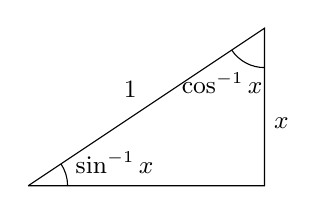
\begin{tikzpicture}[font=\small]
\pgfmathsetmacro{\len}{3}
\pgfmathsetmacro{\h}{2}
\pgfmathsetmacro{\angA}{atan(\h/\len)}
\pgfmathsetmacro{\angB}{90-\angA}
\draw(0,0)--++(\len,0)--++(0,\h)node[pos=0.4,right]{$x$}--(0,0)node[pos=0.5,above left]{$1$};
\RightAngle{(\len,\h)}{(\len,0)}{(0,0)}
\draw[]([shift={(0:0.5)}]0,0) arc (0:\angA:0.5);
\draw(1/2*\angA:0.5)node[right,yshift=1ex]{$\sin^{-1}x$};
\draw([shift={(-90:0.5)}]\len,\h) arc (-90:-90-\angB:0.5);
\draw(\len,\h)++(-90-1/2*\angB:0.5)node[below,xshift=-2ex]{$\cos^{-1}x$};
\end{tikzpicture}
\caption{$\sin^{-1}x+\cos^{-1}x=\frac{\pi}{2}$}
\label{شکل_ماورائی_سائن_کوسائن_تعلق}
\end{minipage}
\end{figure}

\جزوحصہء{\عددی{\tan x}، \عددی{\cot x}، \عددی{\sec x} اور \عددی{\csc x} کے الٹ}
متغیر \عددی{x} کا الٹ ٹینجنٹ وہ زاویہ ہو گا جس کا ٹینجنٹ \عددی{x} ہو۔ اسی طرح \عددی{x} کا الٹ کوٹینجنٹ وہ زاویہ ہو گا جس کا کوٹینجنٹ \عددی{x} ہو۔

\ابتدا{تعریف}
وقفہ \عددی{(-\pi/2,\pi/2)} میں وہ عدد جس کا \عددی{\tan y=x} ہو عدد \عددی{y=\tan^{-1}x} ہو گا۔ اسی طرح وقفہ  \عددی{(0,\pi)} میں وہ عدد جس کا \عددی{\cot y=x} ہو عدد \عددی{y=\cot^{-1}x} ہو گا۔
\انتہا{تعریف}
%=============
ہم کھلا وقفہ لیتے ہیں تا  کہ ان  نقطوں سے نجات حاصل کر سکیں جن پر ٹینجنٹ اور کوٹینجنٹ غیر معین ہیں۔

تفاعل \عددی{y=\tan^{-1}x} کی ترسیم تفاعل \عددی{x=\tan y} کی ترسیم، جو مبدا کے لحاظ سے تشاکلی ہے، کا کچھ حصہ  ہے لہٰذا یہ بھی مبدا کے لحاظ سے تشاکلی ہو گا (شکل \حوالہ{شکل_ماورائی_ترسیم_الٹ_ٹینجنٹ})۔ الجبرائی طور پر اس سے مراد 
\begin{align}
\tan^{-1}(-x)=-\tan^{-1}x
\end{align} 
ہے، یعنی، الٹ ٹینجنٹ طاق تفاعل ہے۔ تفاعل \عددی{y=\cot^{-1}x} کی ترسیم میں ایسی کوئی تشاکلی نہیں پائی جاتی ہے (شکل \حوالہ{شکل_ماورائی_ترسیم_الٹ_کوٹینجنٹ})۔
\begin{figure}
\centering
\begin{minipage}{0.45\textwidth}
\centering
\begin{tikzpicture}[font=\scriptsize,declare function={f(\x)=tan(deg(\x));}]
\pgfmathsetmacro{\k}{pi/2}
\begin{axis}[axis on top,clip=false,small,axis lines=middle,xlabel={$x$},ylabel={$y$},xlabel style={at={(current axis.right of origin)},anchor=west},ylabel style={at={(current axis.above origin)},anchor=south},ytick={-\k,\k},yticklabels={$-\tfrac{\pi}{2}$,$\tfrac{\pi}{2}$},ymax=\k+0.2,ymin=-\k-0.2,xtick={\empty}]
\addplot[domain=-pi/2:pi/2,smooth]({f(x)},x);
\draw(0,\k/2)node[left,xshift=-2ex]{$\begin{aligned} y=\tan^{-1}x\\ (-\infty,\infty)\quad \text{\RL{دائرہ کار}}\\ (-\pi/2,\pi/2)\quad\text{\RL{سعت}} \end{aligned}$};
\end{axis}
\end{tikzpicture}
\caption{ترسیم $y=\tan^{-1}x$}
\label{شکل_ماورائی_ترسیم_الٹ_ٹینجنٹ}
\end{minipage}\hfill
\begin{minipage}{0.45\textwidth}
\centering
\begin{tikzpicture}[font=\scriptsize,declare function={f(\x)=cot(deg(\x));}]
\pgfmathsetmacro{\k}{pi}
\pgfmathsetmacro{\kh}{pi/2}
\begin{axis}[clip=false,small,axis lines=middle,xlabel={$x$},ylabel={$y$},xlabel style={at={(current axis.right of origin)},anchor=west},ylabel style={at={(current axis.above origin)},anchor=south},ytick={\kh,\k},yticklabels={$\tfrac{\pi}{2}$,$\pi$},ymax=\k+0.2,xtick={\empty},ymin=0]
\addplot[domain=0.2:pi-0.2,smooth]({f(x)},x);
\draw(0,3/4*\k)node[right,xshift=2ex]{$\begin{aligned} y=\cot^{-1}x\\ (-\infty,\infty)\quad \text{\RL{دائرہ کار}}\\ 
(0,\pi)\quad\text{\RL{سعت}} \end{aligned}$};
\end{axis}
\end{tikzpicture}
\caption{ترسیم $y=\cot^{-1}x$}
\label{شکل_ماورائی_ترسیم_الٹ_کوٹینجنٹ}
\end{minipage}
\end{figure}

تفاعل \عددی{\sec x} اور \عددی{\csc x} کے محدود روپ کے الٹ کی ترسیمات کو بالترتیب شکل \حوالہ{شکل_ماورائی_ترسیم_الٹ_سیکنٹ} اور شکل \حوالہ{شکل_ماورائی_ترسیم_الٹ_کوسیکنٹ} میں دکھایا گیا ہے۔
\begin{figure}
\centering
\begin{minipage}{0.45\textwidth}
\centering
\begin{tikzpicture}[font=\scriptsize,declare function={f(\x)=sec(deg(\x));}]
\pgfmathsetmacro{\k}{pi}
\pgfmathsetmacro{\kh}{pi/2}
\begin{axis}[axis on top,clip=false,small,axis lines=middle,xlabel={$x$},ylabel={$y$},xlabel style={at={(current axis.right of origin)},anchor=west},ylabel style={at={(current axis.above origin)},anchor=south},ytick={\kh,\k},yticklabels={$\tfrac{\pi}{2}$,$\pi$},xtick={-1,1},enlargelimits=true]
\addplot[domain=0:pi/2-0.3,smooth]({f(x)},x);
\addplot[domain=pi/2+0.3:pi,smooth]({f(x)},x);
\draw(0,3/4*\k)node[right,xshift=2ex]{$\begin{aligned} y=\sec^{-1}x\\ \abs{x}\ge 1\quad \text{\RL{دائرہ کار}}\\
 [0,\pi/2)\cup(\pi/2,\pi]\quad\text{\RL{سعت}} \end{aligned}$};
\draw(-1,pi)node[circ]{}  (1,0)node[circ]{};
\end{axis}
\end{tikzpicture}
\caption{ترسیم $y=\sec^{-1}x$}
\label{شکل_ماورائی_ترسیم_الٹ_سیکنٹ}
\end{minipage}\hfill
\begin{minipage}{0.45\textwidth}
\centering
\begin{tikzpicture}[font=\scriptsize,declare function={f(\x)=cosec(deg(\x));}]
\pgfmathsetmacro{\k}{pi/2}
\begin{axis}[clip=false,small,axis lines=middle,xlabel={$x$},ylabel={$y$},xlabel style={at={(current axis.right of origin)},anchor=west},ylabel style={at={(current axis.above origin)},anchor=south},ytick={-\k,\k},yticklabels={$-\tfrac{\pi}{2}$,$\tfrac{\pi}{2}$},xtick={-1,1},enlargelimits=true]
\addplot[domain=0.4:\k,smooth]({f(x)},x);
\addplot[domain=-0.4:-\k,smooth]({f(x)},x);
\draw(0,1/2*\k)node[left,xshift=-2ex]{$\begin{aligned} y=\csc^{-1}x\\ \abs{x}\ge 1\quad \text{\RL{دائرہ کار}}\\ 
[-\pi/2,0)\cup(0,\pi/2]\quad\text{\RL{سعت}} \end{aligned}$};
\draw(-1,-\k)node[circ]{}  (1,\k)node[circ]{};
\end{axis}
\end{tikzpicture}
\caption{ترسیم $y=\csc^{-1}x$}
\label{شکل_ماورائی_ترسیم_الٹ_کوسیکنٹ}
\end{minipage}
\end{figure}

انتباہ: \quad
متغیر \عددی{x} کی منفی قیمتوں کے لئے \عددی{\sec^{-1}x} کی تعریف پر اتفاق نہیں پایا جاتا ہے۔ہم ربع دوم میں \عددی{\tfrac{\pi}{2}} اور \عددی{\pi} کے بیچ زاویہ لیں گے۔ اس انتخاب کی بنا \عددی{\sec^{-1}x=\cos^{-1}(1/x)} ہو گا اور \عددی{\sec^{-1}x} کے دائرہ کار کے ہر حصہ پر \عددی{\sec^{-1}x} بڑھتا ہوا تفاعل ہو گا۔

\ابتدا{مثال}\شناخت{مثال_ماورائی_کوٹینجنٹ_مخصوص_قیمتیں}\ترچھا{الٹ کوٹینجنٹ \عددی{\tan^{-1}x} کی مخصوص قیمتیں}\\
الٹ کوٹینجنٹ کی مخصوص قیمتوں کا حصول شکل \حوالہ{شکل_مثال_ماورائی_کوٹینجنٹ_مخصوص_قیمتیں} میں دکھایا گیا ہے۔ درج ذیل دیگر قیمتیں بھی اسی طرح حاصل کی جا سکتی ہیں۔
\begin{align*}
\renewcommand{\arraystretch}{2} 
\begin{array}{c|cccccc}
x&\sqrt{3}&1&\tfrac{\sqrt{3}}{3}&-\tfrac{\sqrt{3}}{3}&-1&-\sqrt{3}\\
\hline
\tan^{-1}x&\tfrac{\pi}{3}&\tfrac{\pi}{4}&\tfrac{\pi}{6}&-\tfrac{\pi}{6}&-\tfrac{\pi}{4}&-\tfrac{\pi}{3}
\end{array}
\end{align*}
\انتہا{مثال}
%======================
\begin{figure}
\centering
\begin{subfigure}{0.45\textwidth}
\centering
\begin{tikzpicture}[font=\scriptsize]
\pgfmathsetmacro{\r}{1.35}
\pgfmathsetmacro{\ang}{30}
\draw[-latex](-1.5,0)--(1.5,0)node[right]{$x$};
\draw[-latex](0,-1.4)--(0,1.5)node[above]{$y$};
\draw[opacity=0.5,fill=lgray]([shift={(90:\r)}]0,0) arc (90:270:\r);
\draw([shift={(-90:\r)}]0,0) arc (-90:90:\r);
\draw(0,0)--++(\ang:\r)node[pos=0.5,above left,xshift=1ex]{$2$}coordinate[](kT)--($(0,0)!(kT)!(1.25,0)$)coordinate[](kR)node[pos=0.7,right,xshift=-0.75ex]{$1$};
\draw($(0,0)!0.5!(kR)$)node[below]{$\sqrt{3}$};
\draw[-stealth]([shift={(0:0.5)}]0,0) arc (0:\ang:0.5);
\draw(\ang/2:0.7)node[]{$\tfrac{\pi}{6}$};
\draw(45:\r)node[above right]{$\tan^{-1}\frac{1}{\sqrt{3}}=\tan^{-1}\frac{\sqrt{3}}{3}=\frac{\pi}{6}$};
\draw(-45:\r)node[below right]{$\tan\frac{\pi}{6}=\frac{1}{\sqrt{3}}$};
\end{tikzpicture}
\end{subfigure}\hfill
\begin{subfigure}{0.45\textwidth}
\centering
\begin{tikzpicture}[font=\scriptsize]
\pgfmathsetmacro{\r}{1.35}
\pgfmathsetmacro{\ang}{-60}
\draw[-latex](-1.5,0)--(1.5,0)node[right]{$x$};
\draw[-latex](0,-1.4)--(0,1.5)node[above]{$y$};
\draw[opacity=0.5,fill=lgray]([shift={(90:\r)}]0,0) arc (90:270:\r);
\draw([shift={(-90:\r)}]0,0) arc (-90:90:\r);
\draw(0,0)--++(\ang:\r)node[pos=0.5,below left,xshift=1ex]{$2$}coordinate[](kT)--($(0,0)!(kT)!(1.25,0)$)coordinate[](kR)node[pos=0.7,right,font=\scriptsize,xshift=-0.75ex]{$-\sqrt{3}$};
\draw($(0,0)!0.5!(kR)$)node[above]{$1$};
\draw[-stealth]([shift={(0:0.25)}]0,0) arc (0:\ang:0.25);
\draw(\ang/2:0.5)node[]{$-\tfrac{\pi}{3}$};
\draw(45:\r)node[above right]{$\tan^{-1}(-\sqrt{3})=-\frac{\pi}{3}$};
\draw(-45:\r)node[below right]{$\tan(-\frac{\pi}{3})=-\sqrt{3}$};
\end{tikzpicture}
\end{subfigure}
\caption{الٹ کوٹینجنٹ کی مخصوص قیمتیں (مثال \حوالہ{مثال_ماورائی_کوٹینجنٹ_مخصوص_قیمتیں})۔}
\label{شکل_مثال_ماورائی_کوٹینجنٹ_مخصوص_قیمتیں}
\end{figure}

\ابتدا{مثال}\شناخت{مثال_ماورائی_مثلث_سے_زاویے}
اگر \عددی{\alpha=\sin^{-1}\tfrac{2}{3}} ہو تب \عددی{\cos \alpha}، \عددی{\tan \alpha}، \عددی{\sec \alpha}، \عددی{\csc \alpha} اور \عددی{\cot\alpha} کیا ہوں گے؟

حل:\quad
چونکہ \عددی{\alpha=\sin^{-1}\tfrac{2}{3}} ہے لہٰذا ہم \عددی{\alpha} کو قائمہ مثلث کا ایک زاویہ تصور کرتے ہیں جس کا مخالف ضلع \عددی{2} اور وتر \عددی{3} ہیں۔ مثلث کا تیسرا ضلع (قاعدہ) درج ذیل ہو گا (شکل \حوالہ{شکل_مثال_ماورائی_مثلث_سے_زاویے})۔
\begin{align*}
\sqrt{3^2-2^2}&=\sqrt{9-4}=\sqrt{5}&&\text{\RL{مسئلہ فیثاغورث}}
\end{align*} 
ہم مثلث پر قاعدہ کی لمبائی لکھ کر درج ذیل حاصل کرتے ہیں۔
\begin{align*}
\cos\alpha=\frac{\sqrt{5}}{3},\,\tan\alpha=\frac{2}{\sqrt{5}},\,\sec\alpha=\frac{3}{\sqrt{5}},\, \csc\alpha=\frac{3}{2},\, \cot\alpha=\frac{\sqrt{5}}{2}
\end{align*}
\انتہا{مثال}
%======================
\begin{figure}
\centering
\begin{minipage}{0.45\textwidth}
\centering
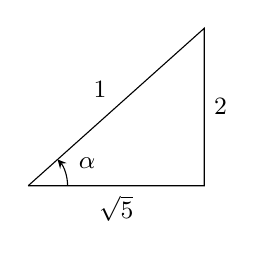
\begin{tikzpicture}[font=\small]
\pgfmathsetmacro{\ang}{asin(2/3)}
\pgfmathsetmacro{\len}{sqrt(5)}
\draw(0,0)--({sqrt(5)},0)node[pos=0.5,below]{$\sqrt{5}$}--++(0,2)node[pos=0.5,right]{$2$}--(0,0)node[pos=0.5,above left]{$1$};
\draw[-stealth]([shift={(0:0.5)}]0,0) arc (0:\ang:0.5);
\draw(\ang/2:0.8)node[]{$\alpha$};
\RightAngle{(\len,2)}{(\len,0)}{(0,0)}
\end{tikzpicture}
\caption{مثلث  کی مدد سے زاویوں کا حصول (مثال \حوالہ{مثال_ماورائی_مثلث_سے_زاویے})}
\label{شکل_مثال_ماورائی_مثلث_سے_زاویے}
\end{minipage}\hfill
\begin{minipage}{0.45\textwidth}
\centering
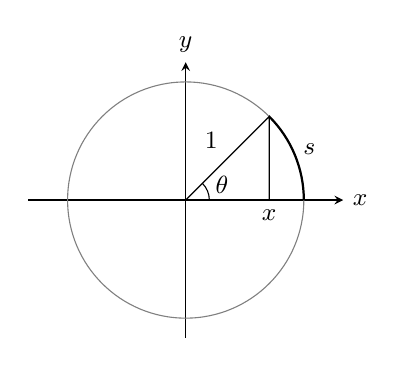
\begin{tikzpicture}[font=\small]
\pgfmathsetmacro{\len}{1.5}
\pgfmathsetmacro{\ang}{45}
\pgfmathsetmacro{\k}{\len*cos(\ang)}
\draw[-stealth](-\len-0.5,0)--(\len+0.5,0)node[right]{$x$};
\draw[-stealth](0,-\len-0.25)--(0,\len+0.25)node[above]{$y$};
\draw[gray](0,0) circle (\len);
\draw(0,0)--++(\ang:\len)node[pos=0.5,above left]{$1$}--(\k,0)node[below]{$x$};
\RightAngle{(\ang:\len)}{(\k,0)}{(0,0)}
\draw[thick] ([shift={(0:\len)}]0,0) arc (0:\ang:\len);
\draw([shift={(0:0.3)}]0,0) arc (0:\ang:0.3);
\draw(\ang/2:0.5)node[]{$\theta$};
\draw(\ang/2:\len+0.2)node[]{$s$};
\end{tikzpicture}
\caption{اکائی دائرہ میں زاویہ \عددی{\theta=\cos^{-1}x} مخالف قوس کی لمبائی \عددی{s} کے برابر ہو گا۔}
\label{شکل_ماورائی_قوس_اور_الٹ_کوسائن}
\end{minipage}
\end{figure}

رداس \عددی{r} کے دائرہ میں مرکز پر زاویہ \عددی{\theta} اور قوس کی لمبائی \عددی{s} کا تعلق \عددی{s=r\theta} ہے لہٰذا  اکائی دائرہ میں \عددی{s=\theta} ہو گا (شکل \حوالہ{شکل_ماورائی_قوس_اور_الٹ_کوسائن})۔ یوں متغیر \عددی{x} کا الٹ کوسائن \عددی{\cos^{-1}x} زاویہ \عددی{\theta}دیگا جس کی قیمت مخالف قوس کی لمبائی \عددی{s} کے برابر ہو گی۔ الٹ سائن کے لئے بھی اس قسم کا تعلق پایا جاتا ہے۔
%=======================
\ابتدا{مثال}\شناخت{مثال_ماورائی_الٹ_تکونیاتی_قیمت_تلاش}
\عددی{\cot\big(\sec^{-1}(-\tfrac{2}{\sqrt{3}})+\csc^{-1}(-2)\big)} کی قیمت تلاش کریں۔

حل:\quad
ہم اندر سے باہر کی جانب چلتے ہوئے زاویوں اور نسبتوں کو مثلثوں  کی مدد سے ظاہر کریں گے۔

\موٹا{پہلا قدم:}\quad
سیکنٹ کی منفی قیمتیں ربع دوم کے زاویوں سے حاصل ہوں گی (شکل \حوالہ{شکل_مثال_ماورائی_الٹ_تکونیاتی_قیمت_تلاش}-ا):
\begin{align*}
\sec^{-1}\big(-\frac{2}{\sqrt{3}}\big)=\sec^{-1}\big(\frac{2}{-\sqrt{3}}\big)=\frac{5\pi}{6}
\end{align*}
\موٹا{دوسرا قدم:}\quad
کوسیکنٹ کی منفی قیمتیں ربع چہارم کے زاویوں سے حاصل ہوں گی (شکل \حوالہ{شکل_مثال_ماورائی_الٹ_تکونیاتی_قیمت_تلاش}-ب):
\begin{align*}
\csc^{-1}(-2)=\csc^{-1}\big(\frac{2}{-1}\big)=-\frac{\pi}{6}
\end{align*}
\موٹا{تیسرا قدم:} \quad
کوٹینجنٹ کی قیمتیں ربع چہارم سے حاصل ہو گی(شکل \حوالہ{مثال_ماورائی_الٹ_تکونیاتی_قیمت_تلاش}-ج):
\begin{align*}
\cot\big(\sec^{-1}(-\tfrac{2}{\sqrt{3}})+\csc^{-1}(-2)\big)&=\cot\big(\frac{5\pi}{6}-\frac{\pi}{6}\big)\\
&=\cot\big(\frac{2\pi}{3}\big)\\
&=-\frac{1}{\sqrt{3}}
\end{align*}
\انتہا{مثال}
%=====================
\begin{figure}
\centering
\begin{subfigure}{0.3\textwidth}
\centering
\begin{tikzpicture}[font=\small]
\pgfmathsetmacro{\ang}{150}
\pgfmathsetmacro{\r}{2}
\pgfmathsetmacro{\kx}{\r*cos(\ang)}
\pgfmathsetmacro{\ky}{\r*sin(\ang)}
\draw[-latex](-2,0)--(0.75,0)node[right]{$x$};
\draw[-latex](0,-0.25)--(0,1.25)node[above]{$y$};
\draw(0,0)--(\kx,0)node[pos=0.5,below]{$-\sqrt{3}$}--++(0,\ky)node[pos=0.5,left]{$1$}--(0,0)node[pos=0.3,above right]{$2$};
\draw[-stealth]([shift={(0:0.5)}]0,0) arc (0:\ang:0.5);
\draw(60:0.8)node[]{$\tfrac{5\pi}{6}$};
\draw(165:0.9)node[]{$\tfrac{\pi}{6}$};
\end{tikzpicture}
\caption{\عددی{\sec(\tfrac{5\pi}{6})=-\tfrac{2}{\sqrt{3}}}}
\end{subfigure}\hfill
\begin{subfigure}{0.3\textwidth}
\centering
\begin{tikzpicture}[font=\small]
\pgfmathsetmacro{\ang}{-30}
\pgfmathsetmacro{\r}{2}
\pgfmathsetmacro{\kx}{\r*cos(\ang)}
\pgfmathsetmacro{\ky}{\r*sin(\ang)}
\draw[-latex](-0.25,0)--(\kx+0.5,0)node[right]{$x$};
\draw[-latex](0,-1.25)--(0,0.5)node[above]{$y$};
\draw(0,0)--(\kx,0)node[pos=0.5,above]{$\sqrt{3}$}--++(0,\ky)node[pos=0.5,right]{$-1$}--(0,0)node[pos=0.5,below left]{$2$};
\draw[-stealth]([shift={(0:0.5)}]0,0) arc (0:\ang:0.5);
\draw(\ang/2:0.9)node[]{$-\tfrac{\pi}{6}$};
\end{tikzpicture}
\caption{\عددی{\csc(-\tfrac{\pi}{6})=-2}}
\end{subfigure}\hfill
\begin{subfigure}{0.3\textwidth}
\centering
\begin{tikzpicture}[font=\small]
\pgfmathsetmacro{\ang}{120}
\pgfmathsetmacro{\r}{2}
\pgfmathsetmacro{\kx}{\r*cos(\ang)}
\pgfmathsetmacro{\ky}{\r*sin(\ang)}
\draw[-latex](-1.25,0)--(0.9,0)node[right]{$x$};
\draw[-latex](0,-0.25)--(0,1.75)node[above]{$y$};
\draw(0,0)--(\kx,0)node[pos=0.5,below]{$-1$}--++(0,\ky)node[pos=0.5,left]{$\sqrt{3}$}--(0,0)node[pos=0.5,above right]{$2$};
\draw[-stealth]([shift={(0:0.5)}]0,0) arc (0:\ang:0.5);
\draw(1/3*\ang:0.9)node[]{$\tfrac{2\pi}{3}$};
\draw(155:0.5)node[]{$\tfrac{\pi}{3}$};
\end{tikzpicture}
\caption{\عددی{\cot(\tfrac{2\pi}{3})=-\tfrac{1}{\sqrt{3}}}}
\end{subfigure}
\caption{مثلث برائے مثال \حوالہ{مثال_ماورائی_الٹ_تکونیاتی_قیمت_تلاش}}
\label{شکل_مثال_ماورائی_الٹ_تکونیاتی_قیمت_تلاش}
\end{figure}

\ابتدا{مثال}\شناخت{مثال_ماورائی_ٹینجنٹ_سے_سیکنٹ}
\عددی{\sec\big(\tan^{-1}\tfrac{x}{3}\big)} تلاش کریں۔

\begin{figure}
\centering
\begin{subfigure}{0.45\textwidth}
\centering
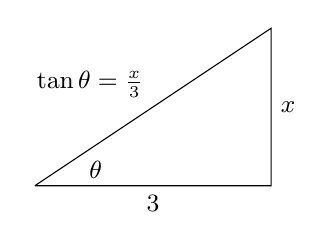
\begin{tikzpicture}[font=\small]
\draw(0,0)--(3,0)node[pos=0.5,below]{$3$}--++(0,2)node[pos=0.5,right]{$x$}--(0,0)node[pos=0.5,above left]{$\tan\theta=\frac{x}{3}$};
\draw(15:0.8)node[]{$\theta$};
\end{tikzpicture}
\caption{}
\end{subfigure}\hfill
\begin{subfigure}{0.45\textwidth}
\centering
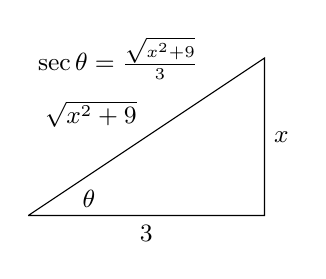
\begin{tikzpicture}[font=\small]
\draw(0,0)--(3,0)node[pos=0.5,below]{$3$}--++(0,2)node[pos=0.5,right]{$x$}--(0,0)node[pos=0.5,above left]{$\sqrt{x^2+9}$};
\draw(15:0.8)node[]{$\theta$};
\draw(0,2)node[right]{$\sec\theta=\frac{\sqrt{x^2+9}}{3}$};
\end{tikzpicture}
\caption{}
\end{subfigure}
\caption{مثلث برائے مثال \حوالہ{مثال_ماورائی_ٹینجنٹ_سے_سیکنٹ}}
\label{شکل_مثال_ماورائی_ٹینجنٹ_سے_سیکنٹ}
\end{figure}

حل:\quad
ہم \عددی{\theta=\tan^{-1}(x/3)} لے کر زاویہ \عددی{\theta} کو قائمہ مثلث میں تصور کرتے ہیں (شکل \حوالہ{شکل_مثال_ماورائی_ٹینجنٹ_سے_سیکنٹ}-ا)۔ یوں
\begin{align*}
\tan\theta=\frac{\text{مخالف}}{\text{قریبی}}=\frac{x}{3}
\end{align*}
ہو گا۔مثلث کا وتر
\begin{align*}
\sqrt{x^2+3^2}&=\sqrt{x^2+9}
\end{align*}
ہو گا لہٰذا سیکنٹ کی قیمت درج ذیل ہو گی (شکل \حوالہ{شکل_مثال_ماورائی_ٹینجنٹ_سے_سیکنٹ}-ب)۔
\begin{align*}
\sec\big(\tan^{-1}\frac{x}{3}\big)&=\sec \theta=\frac{\sqrt{x^2+9}}{3}
\end{align*}
\انتہا{مثال}
%=====================

\حصہء{سوالات}

